\documentclass[10pt,a4paper]{article}
\usepackage[margin=1.9cm]{geometry}
\usepackage[T1]{fontenc}
\usepackage{lmodern}
\usepackage{microtype}
\usepackage{amsmath,amssymb}
\usepackage{booktabs,tabularx,array}
\usepackage{xcolor}
\usepackage{listings}
\usepackage{tikz}
\usetikzlibrary{arrows.meta,positioning,shapes.geometric,fit,backgrounds,calc}
\usepackage{enumitem}
\usepackage[hidelinks]{hyperref}
\setlist{nosep,leftmargin=1.4em}
\definecolor{ink}{HTML}{1F2A44}
\definecolor{acc}{HTML}{0F7B6C}
\definecolor{warn}{HTML}{B5462E}
\definecolor{soft}{HTML}{E8F3F1}
\definecolor{softw}{HTML}{F7E9E5}
\lstset{basicstyle=\ttfamily\footnotesize,columns=fullflexible,keepspaces=true,
  frame=single,rulecolor=\color{black!25},backgroundcolor=\color{black!3},
  keywordstyle=\color{ink}\bfseries,language=C,showstringspaces=false}
\tikzset{
  box/.style={draw=ink,rounded corners=3pt,fill=soft,align=center,font=\small,minimum height=9mm,inner sep=4pt},
  dbox/.style={box,fill=softw,draw=warn},
  arr/.style={-{Stealth[length=2.2mm]},thick,draw=ink},
  lab/.style={font=\scriptsize,text=black!70}}
\emergencystretch=1.5em
\newcommand{\Pz}{P_0}\newcommand{\Po}{P_1}

\usepackage{url}
\def\UrlBreaks{\do\/\do-\do_}
\begin{document}
\thispagestyle{empty}
\vspace*{\fill}
\begin{center}
{\Huge\bfseries Verdicts with Evidence (VWE)}\\[10pt]
{\Large Checking whether an AI-made change to a C function really does what was asked}\\[10pt]
{\normalsize Project report \quad$\cdot$\quad C-Based VLSI Design (CS5291)}\\[10pt]
\textbf{Submitted by}\\[3pt]
\begin{tabular}{@{}c@{}}
Dhruvkumar R Pansuriya (230101071)\\
Aryan Kaushik (230101018)\\
Lasya Madhu Sundar (230101058)
\end{tabular}\\[8pt]
\begin{tabular}{@{}c@{}}
\textbf{Instructor}\\[2pt]
Dr.\ Chandan Karfa
\end{tabular}\\[8pt]
{\large Indian Institute of Technology Guwahati}\\[6pt]
{\small 23 November 2026}\\[4pt]
{\small Code, tests and results:
\url{https://github.com/DhruvPansuriya/C-Based-VLSI-Design-Course-Project}
(branch \texttt{implementation-start})}
\end{center}
\vspace{2pt}
\begin{abstract}
\noindent When an AI assistant is asked to fix a C function, it returns new code. Someone still has
to decide whether that code is right. Our tool, VWE, takes three things: the original buggy
function $\Pz$, the request in plain English $N$, and the new version $\Po$. It answers
\textbf{ACCEPT}, \textbf{REJECT} or \textbf{UNDECIDED}, and it attaches the evidence behind the
answer: either a proof, or a concrete input that shows the problem and that we have run for real.
Since English requests can mean more than one thing, VWE writes down several possible meanings of
$N$, using only $\Pz$ and $N$. It never shows $\Po$ to the language model. It then uses the CBMC
model checker to check two things: that $\Po$ makes the requested change, and that it leaves the
rest of $\Pz$'s behaviour alone. We tested VWE on 181 cases from another course team's project
(we call it Approach-1). VWE gave a decision on 125 of them and agreed with that team's answer on
all 125. On a second benchmark built from public HLS bugs, VWE made no wrong decision, but it
declined to decide almost every case. This report explains how the method works, which tools it
uses, one full example, and what we measured.
\end{abstract}
\vspace*{\fill}
\newpage

\section{The problem}
\label{sec:problem}
There are three easy ways to check AI-written code, and each one has a weakness. Running a few
tests misses rare bugs. Asking another language model ``is this correct?'' is risky, because the
model reads $\Po$ and can be convinced by it. Turning the English request into one formal
specification forces us to pick one meaning, even when the request is ambiguous. VWE does
something different: it keeps several possible meanings of the request, and it only gives a
verdict when the evidence points the same way for all of them.

\begin{center}
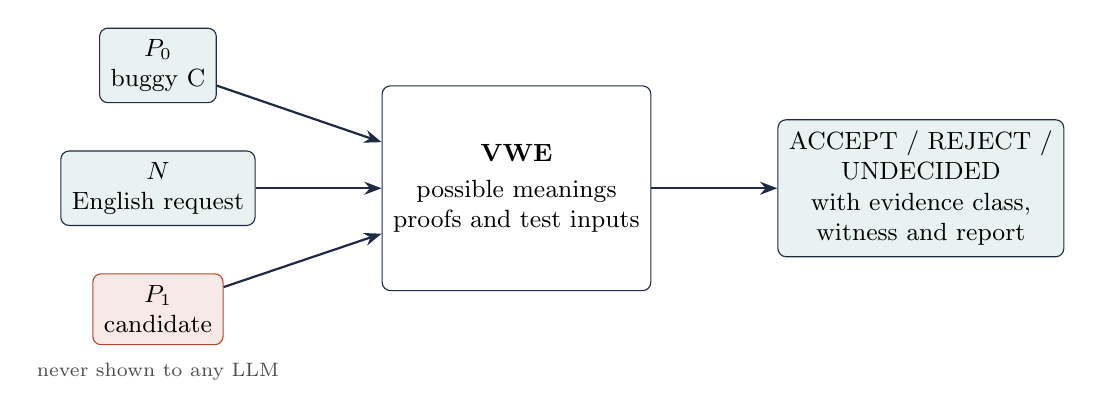
\begin{tikzpicture}[node distance=6mm and 9mm]
\node[box] (p0) {$\Pz$\\buggy C};
\node[box,below=of p0] (n) {$N$\\English request};
\node[dbox,below=of n] (p1) {$\Po$\\candidate};
\node[box,right=16mm of n,minimum width=34mm,minimum height=26mm,fill=white] (vwe) {\textbf{VWE}\\[2pt]possible meanings\\proofs and test inputs};
\node[box,right=16mm of vwe,minimum width=30mm] (out) {ACCEPT / REJECT /\\UNDECIDED\\with evidence class,\\witness and report};
\draw[arr] (p0) -- (vwe); \draw[arr] (n) -- (vwe); \draw[arr] (p1) -- (vwe); \draw[arr] (vwe) -- (out);
\node[lab,below=1mm of p1,align=center] {never shown to any LLM};
\end{tikzpicture}
\end{center}

\paragraph{What the answer means.} Every decision has an \emph{evidence class}.
\textbf{E0} means $\Po$ has a defect we can show without reading $N$ at all, for example a new
out-of-bounds access, or the simulation and synthesis versions of the code behaving differently.
\textbf{E1} means $\Po$ breaks old behaviour in a place that no reasonable reading of $N$ allows
it to change. \textbf{E2} means $\Po$ satisfies (or fails) every meaning of $N$ we kept. If none
of these can be shown, for example because the request is ambiguous or a solver ran out of
time, the answer is \textbf{UNDECIDED}. An ACCEPT always depends on two assumptions that we state
in the report: the declared input range, and that our list of meanings is a fair reading of $N$.

\section{The main ideas}
\begin{enumerate}
\item \textbf{Several readings instead of one specification.} A reading has \emph{clauses} of the
form ``in this zone of inputs, the output must be this'' (for example, ``when $n=0$, return
\texttt{INT\_MIN} and set \texttt{idx} to $-1$''). It also has \emph{Ext}, which says what must hold
outside the zones (usually ``same as $\Pz$''), and a \emph{reach}, the largest set of inputs the
change is allowed to touch. We generate a strict reading, a permissive one, and an adversarial one
that tries to find a different fair meaning.
\item \textbf{The model never sees the answer it is judging.} Readings are built from $N$ and the
signature of $\Pz$ only. If the model could see $\Po$, a wrong $\Po$ could pull the specification
towards itself. The code enforces this: the object that prompts are built from has no place to put
a candidate, and tests plant a marker string in candidates and check it never reaches a prompt.
\item \textbf{The old code is the reference, but only where it is trustworthy.} ``Keep everything
else the same'' only makes sense where $\Pz$ itself is well defined. So, using $\Pz$ alone, VWE
first works out a \emph{reference guard}: the inputs on which $\Pz$ is safe and deterministic.
\item \textbf{If we cannot prove it, we do not decide.} A solver timeout, a loop bound that was not
large enough, the two solvers disagreeing, or a test input that does not reproduce the problem all
lead to UNDECIDED. We prefer saying ``not sure'' to giving a wrong answer.
\end{enumerate}

\section{How VWE works, step by step}
\begin{center}
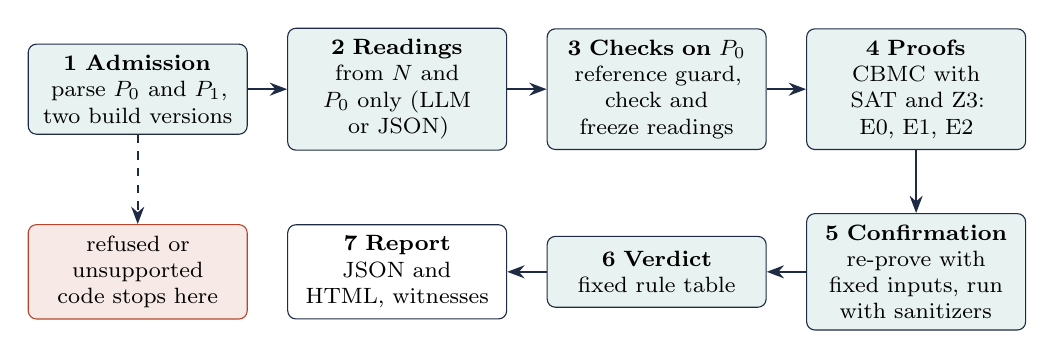
\begin{tikzpicture}[node distance=4.5mm and 5mm,
  st/.style={box,minimum width=27mm,text width=25mm,font=\footnotesize}]
\node[st] (a) {\textbf{1 Admission}\\parse $\Pz$ and $\Po$, two build versions};
\node[st,right=of a] (b) {\textbf{2 Readings}\\from $N$ and $\Pz$ only (LLM or JSON)};
\node[st,right=of b] (c) {\textbf{3 Checks on $\Pz$}\\reference guard, check and freeze readings};
\node[st,right=of c] (d) {\textbf{4 Proofs}\\CBMC with SAT and Z3: E0, E1, E2};
\node[st,below=8mm of d] (e) {\textbf{5 Confirmation}\\re-prove with fixed inputs, run with sanitizers};
\node[st,left=of e] (f) {\textbf{6 Verdict}\\fixed rule table};
\node[st,left=of f,fill=white] (g) {\textbf{7 Report}\\JSON and HTML, witnesses};
\node[st,left=of g,fill=softw,draw=warn] (h) {refused or unsupported code stops here};
\draw[arr] (a)--(b); \draw[arr] (b)--(c); \draw[arr] (c)--(d); \draw[arr] (d)--(e);
\draw[arr] (e)--(f); \draw[arr] (f)--(g); \draw[arr,dashed] (a.south) |- ($(h.north)+(0,2mm)$) -- (h.north);
\end{tikzpicture}
\end{center}

\paragraph{1. Admission} (\texttt{vwe/admission.py}). We preprocess both programs twice: once as
normal C and once with \texttt{\_\_SYNTHESIS\_\_} defined, the way an HLS tool would see it. We
parse them with \texttt{pycparser} and check that the function signature did not change, that
there is nothing we cannot model (such as inline assembly or unknown library calls), and that no
new global variables appeared. If code is refused here, we report it as a policy decision, not as
proof that the fix is wrong.

\paragraph{2. Readings} (\texttt{vwe/interpret.py}, \texttt{vwe/llm/}). Readings come from a
JSON file written by hand, or from a language model. For each model we ask, in order: what kind of
request this is (types T1 to T6), a check of the buffer sizes, then the strict, permissive and
adversarial readings. The adversarial prompt only sees the English summary of the strict reading.
Every reply must be valid JSON in our format; we retry at most twice and record failures. Prompts
have version numbers and hashes, and every call is cached with the model name and seed.

\paragraph{3. Checks that use $\Pz$ only} (\texttt{vwe/regions.py}, \texttt{vwe/validate.py}). First
we find the reference guard by proving that $\Pz$ is safe and deterministic outside some region.
Then each reading is checked before we ever look at $\Po$: V-G, the reading is well typed and has
no undefined behaviour of its own; V-1, its zones are not empty; V-2, $\Pz$ does not already
satisfy it (otherwise it asks for no change); V-3, the parts of $\Pz$ it relies on are well
defined; V-4, for every input there is at least one allowed output (we prove this, we do not just
sample). Readings that fail are dropped. Readings we cannot check either way are kept and block a
final verdict. Equal readings are grouped, and the final set is hashed (``frozen'').

\paragraph{4. Proofs} (\texttt{vwe/harness/}, \texttt{vwe/proof\_jobs.py}). VWE writes a small C test
program, called a harness, that runs $\Pz$ and $\Po$ side by side on the same symbolic inputs.
Buffers get exactly their declared size (\texttt{malloc(n*sizeof(T))}), so an off-by-one read is a
real error. The harness checks:
\[
\text{E0: } \mathit{guard}(x) \Rightarrow \Po(x)\ \text{is safe};\qquad
\text{E1: } x\notin B_{\max} \Rightarrow \bigwedge_k \mathrm{Ext}_k(x,\Pz(x),\Po(x));\qquad
\text{E2: } \Po \text{ satisfies } I_k \text{ for each } k.
\]
CBMC checks each harness twice, once with its SAT solver and once with Z3, and the two must agree.
We always keep the standard safety checks on (array bounds, pointers, overflow, shifts, division)
along with \texttt{--unwinding-assertions} and \texttt{--no-malloc-may-fail}. Calls to
\texttt{abort}, \texttt{exit} and \texttt{longjmp} are replaced with traps so that a candidate
cannot skip a check by exiting early.

\paragraph{5. Confirmation} (\texttt{vwe/replay.py}). When a solver finds a bad input, we fix that
input and prove the failure again. Then we compile both programs with AddressSanitizer and
UndefinedBehaviorSanitizer and actually run them on it. A REJECT needs this real run to agree. A
second model checker, ESBMC, can cancel an ACCEPT if it disagrees, but it can never create one.

\noindent\begin{minipage}[c]{0.40\linewidth}
\paragraph{6. Verdict} (\texttt{vwe/verdict.py}). The verdict is a fixed rule table over the results
of the steps above. It does not call any tool itself. E0 comes first, because it does not depend
on what $N$ means. Anything that was inconclusive on the way turns into UNDECIDED.

\paragraph{7. Report} (\texttt{vwe/report.py}). We write JSON and HTML with the decision, the
evidence class, what kind of claim it is, the assumptions it depends on, the result of every
proof on both solvers, the witness inputs with $\Pz$'s and $\Po$'s outputs, the hash of the frozen
readings and the tool versions.
\end{minipage}\hfill
\begin{minipage}[c]{0.57\linewidth}\centering\small
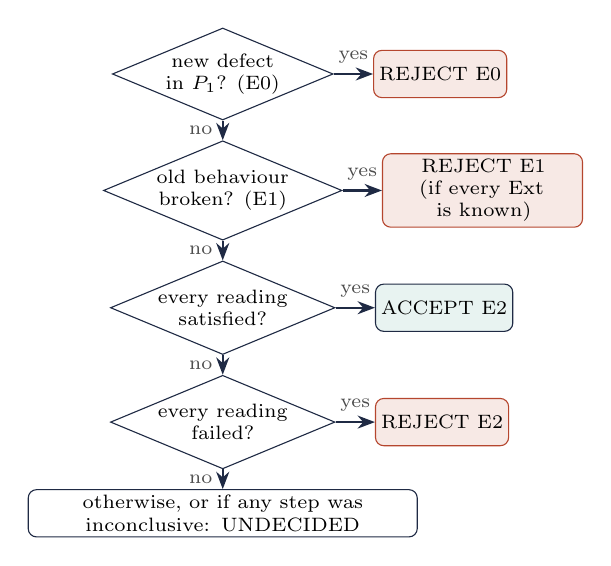
\begin{tikzpicture}[node distance=2.5mm and 5mm,
  q/.style={draw=ink,diamond,aspect=2.4,inner sep=0.5pt,font=\scriptsize,fill=white,align=center},
  r/.style={box,font=\scriptsize,minimum height=6mm,inner sep=2pt}]
\node[q] (q0) {new defect\\in $\Po$? (E0)};
\node[r,fill=softw,draw=warn,right=of q0] (r0) {REJECT E0};
\node[q,below=of q0] (q1) {old behaviour\\broken? (E1)};
\node[r,fill=softw,draw=warn,right=of q1,text width=24mm] (r1) {REJECT E1\\(if every Ext is known)};
\node[q,below=of q1] (q2) {every reading\\satisfied?};
\node[r,right=of q2] (r2) {ACCEPT E2};
\node[q,below=of q2] (q3) {every reading\\failed?};
\node[r,fill=softw,draw=warn,right=of q3] (r3) {REJECT E2};
\node[r,below=2.5mm of q3,fill=white,text width=48mm] (u) {otherwise, or if any step was inconclusive: UNDECIDED};
\foreach \x/\y in {q0/r0,q1/r1,q2/r2,q3/r3} \draw[arr] (\x)--node[lab,above]{yes}(\y);
\foreach \x/\y in {q0/q1,q1/q2,q2/q3,q3/u} \draw[arr] (\x)--node[lab,left]{no}(\y);
\end{tikzpicture}\end{minipage}

\subsection*{How the readings split up the inputs}
Each reading $I_k$ has a change zone $Z_k$ and a reach $R_k$. We combine them into
$B_{\max}=\bigcup_k (Z_k\cup R_k)$, the inputs that \emph{some} reading allows to change. Outside
$B_{\max}$, every reading says ``behave like $\Pz$''. So if $\Po$ behaves differently there, it is
wrong no matter which reading is the right one, and that is the E1 check. Inside the zones, we
check each reading on its own (E2). We only count inputs inside the reference guard, because
$\Pz$ tells us nothing where it has undefined behaviour.
\begin{center}
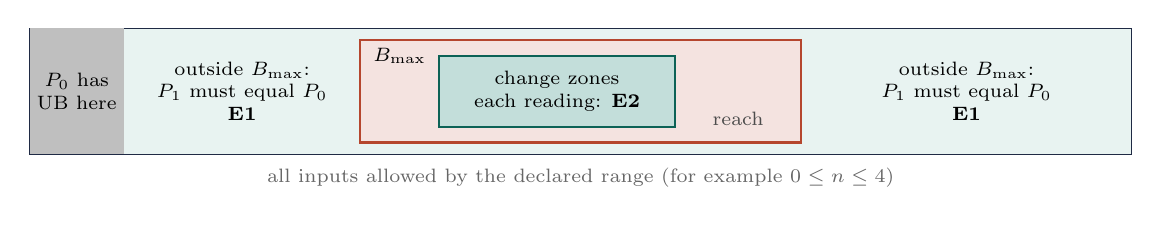
\begin{tikzpicture}[x=1cm,y=1cm]
\fill[soft] (0,0) rectangle (14,1.6);
\draw[ink] (0,0) rectangle (14,1.6);
\fill[warn!15] (4.2,0.15) rectangle (9.8,1.45);
\fill[acc!25] (5.2,0.35) rectangle (8.2,1.25);
\draw[warn,thick] (4.2,0.15) rectangle (9.8,1.45);
\draw[acc!80!black,thick] (5.2,0.35) rectangle (8.2,1.25);
\fill[black!25] (0,0) rectangle (1.2,1.6);
\node[font=\scriptsize,align=center] at (0.6,0.8) {$\Pz$ has\\UB here};
\node[font=\scriptsize,align=center] at (2.7,0.8) {outside $B_{\max}$:\\$\Po$ must equal $\Pz$\\\textbf{E1}};
\node[font=\scriptsize,align=center] at (11.9,0.8) {outside $B_{\max}$:\\$\Po$ must equal $\Pz$\\\textbf{E1}};
\node[font=\scriptsize] at (4.7,1.25) {$B_{\max}$};
\node[font=\scriptsize,text=black!70] at (9.0,0.45) {reach};
\node[font=\scriptsize,align=center] at (6.7,0.8) {change zones\\each reading: \textbf{E2}};
\node[font=\scriptsize,text=black!60] at (7,-0.3) {all inputs allowed by the declared range (for example $0\le n\le 4$)};
\end{tikzpicture}
\end{center}

\subsection*{What a proof harness looks like}
\begin{center}
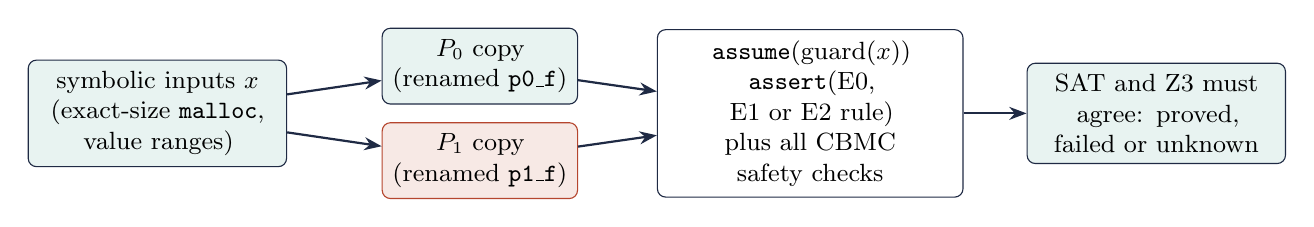
\begin{tikzpicture}[node distance=4mm and 7mm]
\node[box,text width=30mm] (in) {symbolic inputs $x$\\(exact-size \texttt{malloc}, value ranges)};
\node[box,right=12mm of in,yshift=6mm,text width=22mm] (a) {$\Pz$ copy\\(renamed \texttt{p0\_f})};
\node[dbox,right=12mm of in,yshift=-6mm,text width=22mm] (b) {$\Po$ copy\\(renamed \texttt{p1\_f})};
\node[box,right=10mm of a,yshift=-6mm,text width=36mm,fill=white] (as) {\texttt{assume}(guard$(x)$)\\\texttt{assert}(E0, E1 or E2 rule)\\plus all CBMC safety checks};
\node[box,right=8mm of as,text width=30mm] (s) {SAT and Z3 must agree: proved, failed or unknown};
\draw[arr] (in)--(a); \draw[arr] (in)--(b); \draw[arr] (a)--(as); \draw[arr] (b)--(as); \draw[arr] (as)--(s);
\end{tikzpicture}
\end{center}
Both copies get the same inputs, and we compare all their outputs: the return value, every
element written to a buffer, and any global outputs. Loops are unrolled up to a bound. If the bound
is too small, an \emph{unwinding assertion} fails, so a proof can never quietly skip iterations.
We also check that the inputs we assume can actually happen, so a proof is never true just because
nothing was tested.

\section{Where the readings come from}
\begin{center}
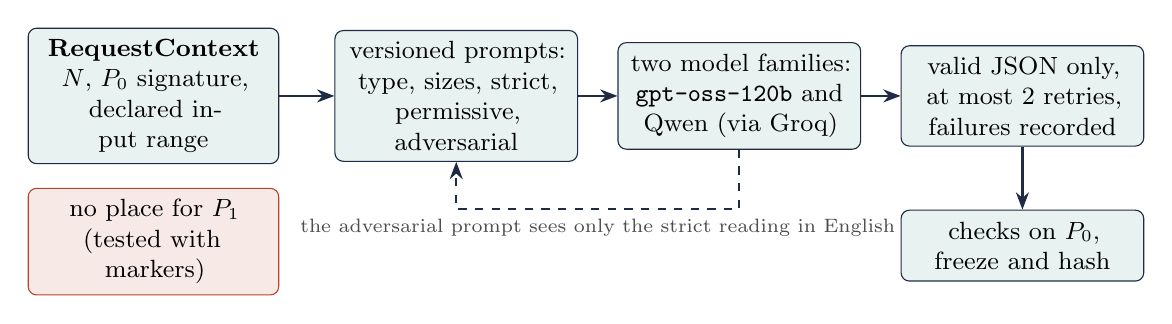
\begin{tikzpicture}[node distance=5mm and 6mm]
\node[box,text width=29mm] (ctx) {\textbf{RequestContext}\\$N$, $\Pz$ signature,\\declared input range};
\node[dbox,below=3mm of ctx,text width=29mm] (no) {no place for $\Po$\\(tested with markers)};
\node[box,right=7mm of ctx,text width=28mm] (pr) {versioned prompts:\\type, sizes, strict,\\permissive, adversarial};
\node[box,right=5mm of pr,text width=28mm] (llm) {two model families:\\\texttt{gpt-oss-120b} and\\Qwen (via Groq)};
\node[box,right=5mm of llm,text width=28mm] (js) {valid JSON only,\\at most 2 retries,\\failures recorded};
\node[box,below=8mm of js,text width=28mm] (fr) {checks on $\Pz$,\\freeze and hash};
\draw[arr] (ctx)--(pr); \draw[arr] (pr)--(llm); \draw[arr] (llm)--(js); \draw[arr] (js)--(fr);
\draw[arr,dashed] (llm.south) |- node[lab,pos=0.75,below]{the adversarial prompt sees only the strict reading in English} ($(pr.south)+(0,-6mm)$) -- (pr.south);
\end{tikzpicture}
\end{center}
A reading is a small JSON file. Its conditions are written in a limited, C-like language with
\texttt{min}, \texttt{max}, \texttt{abs}, bounded \texttt{forall}, \texttt{exists}, \texttt{sum}
and \texttt{count}, plus names like \texttt{out\_ret} for $\Po$'s outputs and \texttt{old\_ret} for
$\Pz$'s. The strict and permissive readings give a narrow and a wide meaning; the adversarial one
looks for another fair meaning under which the strict one would be wrong. A reading passing our
checks does not prove that it matches the English. That is why an ACCEPT is always stated as
conditional on the readings.

\section{A full example: \texttt{argmax}}
\begin{minipage}[t]{0.48\linewidth}
$\Pz$ (it reads \texttt{a[0]} even when $n=0$):
\begin{lstlisting}
int argmax(const int *a,int n,int *idx){
 int m=a[0]; *idx=0;
 for(int i=1;i<n;i++)
   if(a[i]>m){m=a[i];*idx=i;}
 return m; }
\end{lstlisting}
$N$: \emph{``When the array is empty, return \texttt{INT\_MIN} and set \texttt{idx} to $-1$;
otherwise preserve behavior.''} Declared inputs: $0\le n\le 4$, \texttt{a} has $n$ elements,
\texttt{idx} has one, and they do not overlap.
\end{minipage}\hfill
\begin{minipage}[t]{0.49\linewidth}
Candidate $\Po$ (\texttt{v2}):
\begin{lstlisting}
int argmax(const int *a,int n,int *idx){
 if(n==0){*idx=-1;return INT_MIN;}
 int m=a[0]; *idx=0;
 for(int i=1;i<n;i++)
   if(a[i]>=m){m=a[i];*idx=i;}  /* >= */
 return m; }
\end{lstlisting}
The empty case is now handled, but the change from \texttt{>} to \texttt{>=} means the function
now returns the \emph{last} largest element instead of the first.
\end{minipage}

\medskip
\noindent\begin{tabularx}{\linewidth}{@{}lX@{}}\toprule
Step & What VWE found (\texttt{make demo-steps}, 34 seconds on a laptop)\\\midrule
Readings & Strict: when $n=0$, \texttt{out\_ret==INT\_MIN} and \texttt{out\_idx[0]==-1}; elsewhere,
same outputs as $\Pz$. Permissive: the same with $n\le 0$. Both pass all checks and mean the same
thing on these inputs.\\
Reference guard & $\Pz$ has undefined behaviour exactly when $n\le0$ (it reads \texttt{a[0]}), so
the guard is $n>0$.\\
E0 & Proved: \texttt{v2} adds no new undefined behaviour.\\
E1 & Failed. Witness: $n=4$ and all four elements equal to \texttt{INT\_MAX}. $\Pz$ returns
\texttt{idx=0} and $\Po$ returns \texttt{idx=3}. This input is outside every change zone, and every
reading says the result should not change there.\\
Confirmation & The failure repeats with the inputs fixed (SAT and Z3), and a real run under
sanitizers gives the same outputs.\\
Verdict & \textbf{REJECT E1}: old behaviour was broken, whichever reading of $N$ is meant.\\\bottomrule
\end{tabularx}

\smallskip\noindent For comparison, \texttt{v1} (the correct fix) gets ACCEPT E2, and \texttt{v3},
which reads \texttt{a[n]}, gets REJECT E0 with the out-of-bounds read confirmed by AddressSanitizer.
When a request really is ambiguous (our Example~5 asks to ``handle overflow'' without saying whether
to saturate or report an error) and a candidate matches one meaning but not the other, VWE answers
UNDECIDED and shows both readings.

\section{A complete run, stage by stage: saturating addition}
\label{sec:walk}
This section follows one task through the whole pipeline and shows the real output of each stage.
Everything in the grey boxes was copied from an actual run of
\texttt{python scripts/demo\_steps.py --task ex1\_saturate --candidate v3} on 23 November 2026
(16.4 seconds on our laptop). We only shortened long file paths, marked with ``\ldots''.

\paragraph{The inputs.} The original function adds two 8-bit numbers and wraps around on overflow
($200+100$ gives $44$). The request asks for saturation. Candidate \texttt{v3} is a bad fix: it
always returns 255, so it handles overflow but breaks every normal sum.
\begin{lstlisting}[language={}]
P0 (original):  unsigned char add8(unsigned char a, unsigned char b)
                { return (unsigned char)((unsigned)a + (unsigned)b); }
N (request):    Saturate 8-bit unsigned addition at 255 rather than wrapping on overflow.
P1 (v3):        unsigned char add8(unsigned char a, unsigned char b)
                { (void)a; (void)b; return 255u; }
Declared inputs: a and b are any unsigned char (0..255); no buffers.
\end{lstlisting}

\paragraph{Stage 1: admission.}\mbox{}\par
\begin{lstlisting}[language={}]
status: ok  -  structural admission passed; functional, build-view and pragma obligations remain
build views differ: False;  HLS pragmas seen: 0
\end{lstlisting}
Both programs parse, the signature is the same, and nothing unsupported is used.

\paragraph{Stage 2: readings.} The run uses our two handwritten readings:
\begin{lstlisting}[language={}]
- ex1_saturate.strict: Saturate overflow and preserve ordinary addition.
    when a + b > 255:  out_ret == 255
    elsewhere: out_ret == min(a + b, 255)    reach: a + b > 255
- ex1_saturate.permissive: Any implementation returning the saturated sum is allowed.
    when a + b > 255:  out_ret == min(a + b, 255)
    elsewhere: out_ret == min(a + b, 255)    reach: a + b > 255
\end{lstlisting}
For comparison, this is what the two live models wrote for the same request when given only $N$
and the signature of $\Pz$ (all 10 calls returned valid JSON on the first try):
\begin{lstlisting}[language={}]
groq_gptoss.strict      when a + b > 255: out_ret == 255   ext: out_ret == old_ret   reach: a + b > 255
groq_gptoss.permissive  when a + b > 255: out_ret == 255   ext: out_ret == old_ret   reach: a + b > 255
groq_gptoss.adversarial when a + b > 255: out_ret == 255;  when a + b <= 255: out_ret == a + b
                        ext: unknown   reach: true
groq_qwen.strict / permissive / adversarial
                        when a + b > 255: out_ret == 255   ext: out_ret == old_ret   reach: a + b > 255
\end{lstlisting}
Both models understood the request: change only the overflow case and keep the rest. The models
said ``same as old'' (\texttt{old\_ret}) where we wrote \texttt{min(a+b,255)}; on these inputs
they mean the same thing.

\paragraph{Stage 3a: reference regions on $\Pz$ alone.}\mbox{}\par
\begin{lstlisting}[language={}]
proposed UB region: false   exact UB region: false
certified safe reference guard: !(false)
\end{lstlisting}
Unsigned addition never has undefined behaviour, so $\Pz$ can be trusted on every input (the guard
is ``not false'', that is, always true).

\paragraph{Stage 3b: checking and freezing the readings (before $\Po$ is looked at).}\mbox{}\par
\begin{lstlisting}[language={}]
ex1_saturate.permissive: valid  (V-4: joint output tuple proved for every modeled input)
ex1_saturate.strict: valid  (V-4: joint output tuple proved for every modeled input)
equivalence classes: [['ex1_saturate.permissive', 'ex1_saturate.strict']]
frozen set sha256: 50973ac285e940f1...
\end{lstlisting}
Both readings pass every check, and VWE proves they mean the same thing on these inputs, so only
one of them has to be checked against $\Po$ later.

\paragraph{Stage 4a: proof E0, new undefined behaviour?}\mbox{}\par
\begin{lstlisting}[language={}]
Proof: candidate safety on reference guard
outcome: PROVED   backends: sat=success, z3=success
Proof: reference on common keep region          (is P0 deterministic where it must be kept?)
outcome: PROVED   backends: sat=success, z3=success
\end{lstlisting}

\paragraph{Stage 4b: proof E1, is old behaviour kept outside the change zone?} The change zone of
both readings is $a+b>255$. Outside it, $\Po$ must return what $\Pz$ returns. This is the key line
of the generated harness (\texttt{e1/main.c}); \texttt{\_\_vwe\_zero} is $\Pz$'s result and
\texttt{\_\_vwe\_one} is $\Po$'s:
\begin{lstlisting}[language={}]
unsigned char __vwe_in_scalar_0_0=nondet___vwe_0();
__CPROVER_assume(0LL <= __vwe_in_scalar_0_0 && __vwe_in_scalar_0_0 <= 255LL);
...
__CPROVER_assert(((__vwe_zero.r0==__vwe_one.r0)) || vwe_observer_1(...) || vwe_observer_2(...),
                 "VWE.E1.preservation");
\end{lstlisting}
It is checked with this command (the same flags on every CBMC run), once with the SAT solver and
once with Z3:
\begin{lstlisting}[language={}]
cbmc .../checked.goto --bounds-check --pointer-check --div-by-zero-check
     --signed-overflow-check --undefined-shift-check --pointer-primitive-check
     --unwinding-assertions --no-self-loops-to-assumptions --no-malloc-may-fail
     --json-ui --trace --unwind 9 --no-library
\end{lstlisting}
A quick native random test suggested a bad input first, and both solvers then proved it:
\begin{lstlisting}[language={}]
Proof: pre-pass preservation hint
outcome: VIOLATED   backends: sat=failure, z3=failure
note: e1: main.assertion.1 VWE.E1.preservation
witness inputs: {'a': '0', 'b': '0'}
  P0 output: {'ret': '0'}   P1 output: {'ret': '255'}
\end{lstlisting}
For $a=b=0$ there is no overflow, so every reading says the answer must stay $0$, but \texttt{v3}
returns $255$.

\paragraph{Stage 5: confirmation.}\mbox{}\par
\begin{lstlisting}[language={}]
Proof: counterexample with fixed inputs 0
outcome: VIOLATED   backends: sat=failure, z3=failure
witness inputs: {'a': '0', 'b': '0'}
Native witness replay
witness 0: confirmed  -  captured observations match the fixed solver witness
\end{lstlisting}
With the inputs fixed to $(0,0)$ both solvers still find the failure. Then both programs were
compiled with AddressSanitizer and UBSan and run in a sandbox (no network, no file writes, 5-second
CPU limit). The recorded outputs were $\Pz=0$ and $\Po=255$, the same as the solver said.

\paragraph{Stages 6 and 7: verdict and report.}\mbox{}\par
\begin{lstlisting}[language={}]
REJECT  E1   claim: repair_correctness
reason: regression outside B_max rejected by every Ext
conditional on: Within the declared caller profile, the witness lies outside the validated
                scope union and its change is rejected by every surviving extended relation.
witness: {'a': '0', 'b': '0'}  (replayed natively: True)
\end{lstlisting}
The HTML report in the run folder lists every proof with both solvers' results, the witness, both
programs' outputs, the frozen reading hash and the tool versions (CBMC 6.11.0, Z3 5.4.1; ESBMC was
not installed on this machine).

\paragraph{The same task with the correct fix.} Running candidate \texttt{v1}, which returns
\texttt{s>255u ? 255u : s}, takes 20.3 seconds and goes down the other path:
\begin{lstlisting}[language={}]
Proof: candidate safety on reference guard              PROVED   sat=success, z3=success
Proof: preservation or Ext outside scope union          PROVED   sat=success, z3=success
Proof: scope agreement for each reading                 PROVED   (both readings)
Proof: class path reachability (zone can be reached)    PROVED
Proof: interpretation ex1_saturate.permissive           PROVED   sat=success, z3=success
ACCEPT  E2   claim: repair_correctness
reason: satisfies every interpretation
readings satisfied: ['ex1_saturate.permissive', 'ex1_saturate.strict']
\end{lstlisting}
Here every check passes, including the one that the overflow zone can actually be reached (so the
proof is not empty), and VWE accepts, stating that this holds for the declared inputs and assuming
the readings are a fair reading of $N$.

\section{Tools we use}
\noindent\begin{tabularx}{\linewidth}{@{}l>{\raggedright\arraybackslash}X@{}}\toprule
Tool (version) & What it does for us\\\midrule
CBMC 6.11.0 & A bounded model checker for C. It turns a harness into a logic formula and either
proves every assertion or gives an input that breaks one. This is our main verifier.\\
SAT solver and Z3 5.4.1 & The two solvers CBMC can use. We run both and only trust a result when
they agree.\\
\texttt{goto-cc}, \texttt{goto-instrument} & CBMC's compiler and program rewriter. We use them to
build the program and to replace \texttt{abort}, \texttt{exit} and \texttt{longjmp} with traps.\\
ESBMC 8.7.0 & A second model checker, used only to double-check an ACCEPT. It runs in our Linux
CI.\\
Clang or GCC with ASan and UBSan & We compile and run every witness for real, so no REJECT is based
only on a solver's trace. We also use them for quick random testing that only gives hints.\\
pycparser, Lark & Parsing C (admission, renaming, signatures) and parsing our reading language.\\
LLMs on Groq: gpt-oss, Qwen & Writing readings from $N$ and $\Pz$'s signature. An OpenAI connection
is also written but was not used because the account had no credit.\\
Python, pytest, GitHub Actions & Everything else: 434 automatic tests, run on every push.\\\bottomrule
\end{tabularx}

\section{What we built}
\begin{center}\small
\noindent\begin{tabularx}{\linewidth}{@{}l>{\raggedright\arraybackslash}X@{}}\toprule
Part & What it includes\\\midrule
Core checker (T00 to T11) & admission, the reading language, the harness generator, the CBMC
jobs, the $\Pz$-only checks, the verdict rules, real runs of witnesses, reports, 20 test cases from
the seven examples in our design document, and two demos.\\
Model layer (T12 to T14) & one client for all model providers (JSON checks, retries, cache, records,
rate-limit handling), versioned prompts, the \texttt{vwe interpret} and \texttt{verify --auto}
commands, and repeated runs to measure stability. Working live with two model families.\\
Evaluation (T15 to T18) & 20 tasks built from the public Chrysalis-HLS bug dataset, candidate
fixes, correct/incorrect labels, three simpler checkers to compare against, and the statistics.\\
Approach-1 evaluation & VWE run on the other team's 181 cases (Section~\ref{sec:approach1}).\\
Not done & the HLS pragma checks and real synthesis numbers (T19, T20), the FIFO extension (T21),
and proofs of the theorems in our design document.\\\bottomrule
\end{tabularx}\end{center}

\section{How we tested it}
\begin{center}
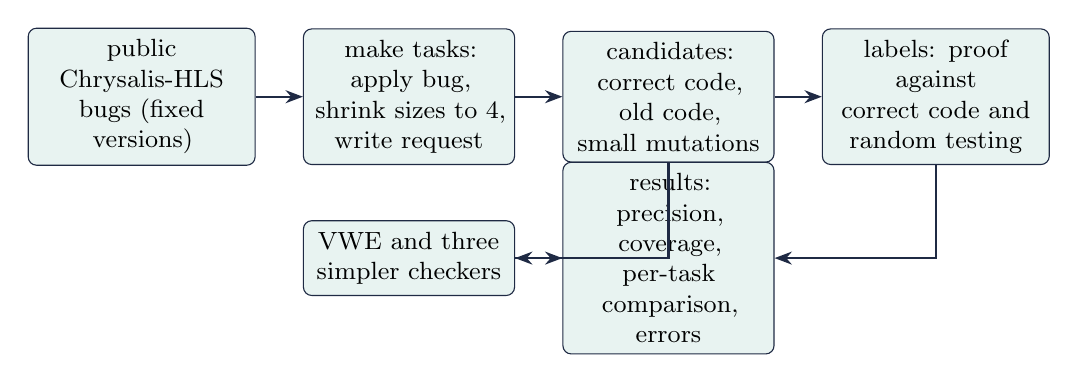
\begin{tikzpicture}[node distance=4mm and 6mm]
\node[box,text width=26mm] (src) {public Chrysalis-HLS\\bugs (fixed versions)};
\node[box,right=of src,text width=24mm] (ad) {make tasks: apply bug,\\shrink sizes to 4,\\write request};
\node[box,right=of ad,text width=24mm] (pool) {candidates:\\correct code, old code,\\small mutations};
\node[box,right=of pool,text width=26mm] (lab) {labels: proof against\\correct code and\\random testing};
\node[box,below=7mm of ad,text width=24mm] (sys) {VWE and three\\simpler checkers};
\node[box,right=of sys,text width=24mm] (met) {results: precision,\\coverage, per-task\\comparison, errors};
\draw[arr] (src)--(ad); \draw[arr] (ad)--(pool); \draw[arr] (pool)--(lab);
\draw[arr] (pool.south) |- (sys.east); \draw[arr] (sys)--(met); \draw[arr] (lab.south) |- (met.east);
\end{tikzpicture}
\end{center}
We made the labels separately and only matched them with VWE's answers at the end. A candidate is
labelled \emph{correct} only if a bounded proof shows it gives the same outputs as the known
correct code, and 10{,}000 random and edge-case runs under sanitizers agree. It is \emph{incorrect}
if we have a confirmed input where it differs. Otherwise it is \emph{unknown} and left out (we
still count these). Candidates from the same task are related, so our confidence intervals
resample whole tasks, and we compare against the simpler checkers task by task. We did not build
the ``ask an LLM to judge'' checker, because it would have to show $\Po$ to a model.

\section{Results}
\subsection{The test sets at a glance}
We used three groups of test cases. All times are wall-clock times on one laptop (Apple M-series,
8 cores, 8 GB RAM) with CBMC 6.11 and Z3 5.4.1, a 120-second limit per solver call in the
benchmark runs, and the default 600 seconds in the example runs.
\begin{center}\small
\noindent\begin{tabularx}{\linewidth}{@{}>{\raggedright\arraybackslash}p{2.0cm}>{\raggedright\arraybackslash}X r >{\raggedright\arraybackslash}p{2.0cm} >{\raggedright\arraybackslash}p{2.8cm}@{}}\toprule
test set & how the cases were made & cases & time per case & result\\\midrule
Golden examples & written by us from the seven examples in our design document; each verdict
was worked out by hand before running & 20 & about 9 s (whole suite 3 min 4 s) & 20 of 20 match the
expected verdict\\
Demo & 9 rows taken from the golden examples with smaller input sizes (K=2) & 9 & 0.6 to 32.8 s
(total 65 s) & 9 of 9 match\\
Chrysalis-HLS & 20 tasks from a public HLS bug dataset; candidates are the correct code, the
unchanged buggy code and small mutations; labels from a proof plus random testing & 97 (89
labelled) & median 7.3 s, mean 45.8 s, max 367 s & 1 decided, correct; 0 wrong\\
Approach-1 & the other team's kernels: their rewrites, their one-bit faults and their 80
subtle-fault cases, with their labels & 181 & median 17.7 s if decided, about 248 s if not & 125
decided, all agree; 0 wrong\\
Live readings & Examples 1, 2 and 4 with readings written by two live models instead of by us & 10
& like the golden cases & 3 same, 7 undecided, 0 opposite\\\bottomrule
\end{tabularx}\end{center}

\subsection{Golden examples (our own test cases)}
These are the seven examples from our design document, turned into runnable tasks with 2 to 5
candidate fixes each. We decided the right answer for every candidate by hand before running VWE.
They are regression tests for the tool, not a measure of accuracy. All 20 match.
\begin{center}\small
\begin{tabular}{@{}lll@{}}\toprule
example & what it tests & VWE verdicts (candidates in order)\\\midrule
1 saturating add & a clear change request & ACCEPT, ACCEPT, REJECT E1, REJECT E2, REJECT E2\\
2 argmax & empty array, old UB, tie-break & ACCEPT E2, REJECT E1, REJECT E0\\
3 rounded average & readings disagree on scope & UNDECIDED, ACCEPT E2, REJECT E2\\
4 sum & off-by-one, exact buffer size & ACCEPT E2, REJECT E0\\
5 32-bit add & ambiguous request & UNDECIDED, UNDECIDED, REJECT E2\\
6 copy overflow & making unsafe code safe & ACCEPT E2, REJECT E1\\
7 build views & simulation vs synthesis build & REJECT E0, ACCEPT E2\\\bottomrule
\end{tabular}\end{center}
The demo runs nine of these with smaller sizes: correct saturation 20.6 s, ``always 255'' 16.6 s,
tie-break regression 26.6 s, new out-of-bounds read 24.1 s, include the last element 32.8 s, read
one past the buffer 24.8 s, ambiguous overflow 23.7 s, build views 8.2 s, and an early-exit check
0.6 s: 65.2 s in total, all nine as expected.

\subsection{Chrysalis-HLS tasks}
\paragraph{How we made the tasks.} Chrysalis-HLS is a public dataset (Apache-2.0) of bugs injected
into HLS benchmark code from MachSuite, CHStone, H.264, the Vitis HLS examples and others. Each bug
comes with the original code and the change that injects it. Our script downloads a fixed version
of the dataset, keeps bugs that are a single edit of a supported type (out-of-bounds, uninitialised
read, bad shift, infinite loop, sign extension, wrong zero initialiser, loop-unrolling mistake),
applies the edit to get $\Pz$, and keeps the original as the correct code. Because CBMC needs small
sizes, it sets every size constant to 4 and limits inputs to $[-1000,1000]$. It drops anything that
does not compile on its own or whose correct version already crashes after shrinking. The request
text comes from a fixed sentence per bug type, so these requests are not written by people. 20 tasks
from 10 different functions remained, out of about 1{,}860 candidates in the dataset.

\paragraph{How we made the candidates and labels.} Each task has the correct code, the unchanged
buggy code, and up to four small mutations of the correct code (a comparison flipped, a constant
changed by one, an \texttt{if} condition removed). That gives 97 candidates. The labels came out as
23 correct, 66 incorrect and 8 unknown, and the proof and the random testing never disagreed. The
model readings for these tasks were written live by \texttt{gpt-oss-120b} and Qwen; five tasks are
missing some gpt-oss readings because we hit Groq's free daily limit.

\paragraph{Time.} VWE: median 7.3 s per candidate, mean 45.8 s, slowest 367 s (slow cases are SAT
timeouts). Tests only: 4.1 s mean. Strict reading only: 12.8 s mean. Regression only: 5.5 s mean.
The whole run took about 1.8 machine-hours with two parallel workers. Checking that the correct
code is never rejected took 441 s for all 20 tasks.

\paragraph{Results.}
\begin{center}\small
\begin{tabular}{@{}lrrrl@{}}\toprule
checker & decided & share & wrong & comment\\\midrule
VWE & 1 & 0.01 & \textbf{0} & one correct REJECT E0 (a new out-of-bounds pointer access)\\
B1, tests only & 89 & 1.00 & 41 & code that does not crash is not always correct\\
B3, strict reading only & 1 & 0.01 & 0 & declines the same cases as VWE\\
B4, regression only & 43 & 0.48 & 10 & misses changes inside the change zone\\\bottomrule
\end{tabular}\end{center}
\noindent VWE declined most cases for two reasons. For 54 candidates we could not establish the
reference guard on $\Pz$, mostly because the SAT solver timed out or a loop needed more unrolling
than allowed. For 36, no reading survived: once the programs were shrunk, the injected bug often had
no visible effect, so check V-2 rightly removed every reading that said ``$\Pz$ must change''. Task
by task, VWE made fewer wrong decisions than the tests-only checker on 12 of the 20 tasks and more on
none (sign test, $p<0.001$), and fewer than the regression-only checker on 5 tasks and more on none.

\subsection{Approach-1 cases}
181 candidates from the other team's project: 51 rewrites, 50 one-bit faults and 80 subtle-fault
cases. VWE decided 125 and agreed with their answer on all 125. A decided case took a median of
17.7 s; cases that ended undecided took about 248 s, almost all of it waiting for solver timeouts.
The full run took about 4.1 machine-hours with three parallel workers. Section~\ref{sec:approach1}
gives the details.

\subsection{Readings from live models compared with ours}
We reran Examples 1, 2 and 4 with readings written by the two live models instead of by us. 3 of
the 10 verdicts stayed the same; the other 7 became UNDECIDED, and none turned into the opposite
answer. In one case the adversarial reading left ``outside the zone'' unspecified; in another, a
reading used a pointer inside a condition, which our reading language cannot evaluate. The model
readings never caused a wrong answer, but they lowered how often VWE could decide.

\section{How VWE did on the Approach-1 cases}
\label{sec:approach1}
\textbf{Approach-1} is the other course team's project, which we received as a zip file. In their
setup, an LLM rewrites a C kernel to get better hardware. Their checker, which combines their own
symbolic execution and Z3 with ESBMC, proves that the rewrite still computes the same thing. Only
proved rewrites go on to high-level synthesis, where they measure area and latency. Their test set
has two parts. The \emph{main set} has 51 kernels, each with a correct rewrite and a version with
one output bit flipped on purpose. The \emph{subtle-fault set} has 80 cases with their own labels:
54 not equivalent, 20 equivalent, and 6 where the new code has undefined behaviour.

\paragraph{How we ran VWE on them.} Each kernel became a VWE task with request type T5, ``improve the
hardware without changing behaviour''. No language model was needed: the only reading is ``every
output equals the original's'', with no change zone. So E1 decides everything except new undefined
behaviour, which is E0. We changed two things and recorded them per task: we replaced
\texttt{<stdint.h>} with plain type definitions, and we raised the size bound to 32 and the loop
bound to 40, because their arrays and loops go up to 32. We kept their files outside our repository,
and we only matched their labels after all of VWE's answers were done. We did not rerun their
checker; we used the results they recorded.

\begin{center}
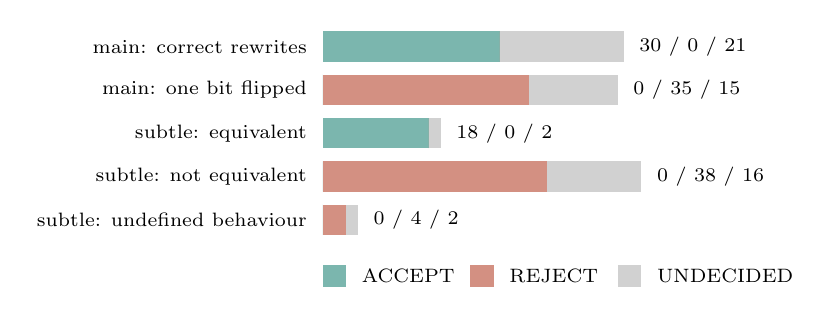
\begin{tikzpicture}[x=0.075cm,y=0.55cm]
\def\bar#1#2#3#4#5{% y, label, accept, reject, undecided
  \fill[acc!55] (0,#1) rectangle ++(#3,0.7);
  \fill[warn!60] (#3,#1) rectangle ++(#4,0.7);
  \fill[black!18] (#3+#4,#1) rectangle ++(#5,0.7);
  \node[anchor=east,font=\scriptsize] at (-1,#1+0.35) {#2};
  \node[anchor=west,font=\scriptsize] at (#3+#4+#5+1,#1+0.35) {#3 / #4 / #5};}
\bar{4}{main: correct rewrites}{30}{0}{21}
\bar{3}{main: one bit flipped}{0}{35}{15}
\bar{2}{subtle: equivalent}{18}{0}{2}
\bar{1}{subtle: not equivalent}{0}{38}{16}
\bar{0}{subtle: undefined behaviour}{0}{4}{2}
\fill[acc!55] (0,-1.2) rectangle ++(4,0.5); \node[anchor=west,font=\scriptsize] at (5,-0.95) {ACCEPT};
\fill[warn!60] (25,-1.2) rectangle ++(4,0.5); \node[anchor=west,font=\scriptsize] at (30,-0.95) {REJECT};
\fill[black!18] (50,-1.2) rectangle ++(4,0.5); \node[anchor=west,font=\scriptsize] at (55,-0.95) {UNDECIDED};
\end{tikzpicture}
\end{center}

\begin{center}\small
\begin{tabular}{@{}lrrrrl@{}}\toprule
group (their label) & cases & ACCEPT & REJECT & UNDECIDED & VWE evidence\\\midrule
main: correct rewrite & 51 & 30 & 0 & 21 & E2\\
main: one bit flipped & 50 & 0 & 35 & 15 & E1 (input run for real)\\
subtle: equivalent change & 20 & 18 & 0 & 2 & E2\\
subtle: real bug & 54 & 0 & 38 & 16 & E1\\
subtle: undefined behaviour & 6 & 0 & 4 & 2 & E0 (confirmed by sanitizer)\\\midrule
total & 181 & 48 & 77 & 56 & 125 decided, \textbf{0 disagreements}\\\bottomrule
\end{tabular}\end{center}

\paragraph{Bugs their tests missed.} Approach-1's report lists five bugs that got past their 264
test inputs and were only found by their proof. VWE rejected all five, each with a concrete input
that both solvers confirmed and that we ran under sanitizers:
\begin{center}\small
\begin{tabular}{@{}lll@{}}\toprule
case & their description & VWE\\\midrule
\texttt{all\_equal16} & differences cancel out under XOR & REJECT E1\\
\texttt{clamp16} & the clamp kicks in one value too early & REJECT E1\\
\texttt{threshold\_pack8} & a rare equality case & REJECT E1\\
\texttt{search\_count16} & one lane repeats another lane's comparison & REJECT E1\\
\texttt{fault\_rare\_magic} & a rare special-case input & REJECT E1\\\bottomrule
\end{tabular}\end{center}

\paragraph{Why VWE did not decide 56 cases.}
\begin{itemize}
\item \textbf{48 cases: no reference guard.} In 32 of the 34 tasks involved, the SAT solver hit the
120-second limit while checking that $\Pz$ is deterministic. These are kernels with a lot of
multiplication (dot products, matrix multiply, matrix--vector, convolution). Since VWE needs both
solvers to agree, one timeout is enough to stop it. A decided case took 17.7 seconds (median); an
undecided one took about 248 seconds.
\item \textbf{5 cases:} the SAT solver timed out on a later check.
\item \textbf{3 cases: a false alarm from CBMC that VWE caught.} On \texttt{gaussian5}, CBMC's
experimental check for uninitialised variables said a local array \texttt{horizontal[15]} was read
before being written. In fact a loop fills all 15 elements first. Re-proving with fixed inputs gave
the same false alarm, but the real run under sanitizers found nothing, so VWE said UNDECIDED
instead of wrongly rejecting a correct rewrite. This is the reason the confirmation step exists.
\end{itemize}

\paragraph{The two approaches compared.}
\begin{center}\small
\noindent\begin{tabularx}{\linewidth}{@{}l>{\raggedright\arraybackslash}X>{\raggedright\arraybackslash}X@{}}\toprule
 & Approach-1 (their checker) & VWE (our project)\\\midrule
question & does the rewrite compute the same thing as the original? & does $\Po$ do what $N$ asks, and leave the rest unchanged?\\
specification & full equivalence, fixed & readings of $N$; here, ``no change in behaviour''\\
engine & their own symbolic execution with Z3, then ESBMC/Z3 on what is left & generated harnesses checked by CBMC with both SAT and Z3\\
confirmation & re-checking the SMT result, compiled-C tests, RTL simulation & re-proof with fixed inputs, real runs with sanitizers; ESBMC can only cancel an ACCEPT\\
cases decided & 181 of 181 (their records) & 125 of 181 (our laptop, 120 s limit)\\
wrong answers & none against its labels & none against the same labels\\
other features & HLS synthesis and area, latency and timing numbers (Bambu, Yosys, OpenSTA) & requests that ask for a real behaviour change, and ambiguous requests; no hardware numbers\\\bottomrule
\end{tabularx}\end{center}
On every case VWE decided, it gave the same answer as Approach-1, using a different engine and no
language model. It decided fewer cases with the time limit we used. Approach-1 also measures the
hardware, which VWE does not. VWE can also check requests that are meant to change behaviour,
which a pure equivalence checker cannot.

\section{Where we stand, in short}
\begin{itemize}
\item \textbf{No wrong answers so far.} Across every evaluation, none of VWE's decisions was
wrong, and there was no wrong E0 or E1 verdict, which the design says should be impossible.
\item \textbf{The cost is undecided cases.} VWE decides often when the request is precise (69\% on
Approach-1) and rarely on our shrunk Chrysalis bugs, where the bug often disappears. The biggest
limit is solver time: the SAT solver is slow on 32- and 64-bit multiplication, while Z3 usually
finishes.
\item \textbf{Keeping $\Po$ away from the model works.} Readings from two different model families
never saw a candidate, and when the models made mistakes, VWE declined to decide instead of giving
a wrong answer.
\item \textbf{Limits we are aware of.} All results hold for the declared input ranges only. The
Chrysalis requests are generated from a template, not written by people. Part of our labelling
uses the same checker, although random testing cross-checks it. We have not measured any hardware,
and the theorems in our design document are not proved.
\end{itemize}

\section{Future work}
\begin{itemize}
\item \textbf{More decisions on arithmetic-heavy code.} Most undecided cases come from the SAT
solver timing out on multiplication. We want to try longer limits, and to check whether Z3 alone
can be trusted for the determinism step on $\Pz$, so one slow solver does not block everything.
\item \textbf{A better uninitialised-memory check.} CBMC's experimental check gave a false alarm on
a loop-filled array. We want an element-by-element check that we have tested properly.
\item \textbf{Smarter handling of unknown parts of readings.} A reading that covers every input
with its zones never uses its ``outside'' rule, so leaving that rule unknown should not block a
verdict. This needs a careful argument and tests before we change the verdict rules.
\item \textbf{Requests written by people.} Our Chrysalis requests come from templates. A set of
real, human-written fix requests would say much more about how well the readings capture intent.
\item \textbf{Hardware side.} Check HLS pragmas (for example that a pipeline or dependence pragma is
safe) and measure area and latency with an HLS tool, as Approach-1 does.
\item \textbf{Larger inputs.} Grow the size bounds, or prove that results for small sizes carry over
to larger ones.
\end{itemize}

\section{Conclusion}
We built VWE, a tool that checks whether an AI-made change to a C function does what an English
request asked, and gives evidence for every answer. It keeps several readings of the request, never
lets the language model see the code it is judging, checks both the change and everything that
should stay the same, and confirms every failure by running it for real. Across our own examples,
a public bug dataset and the other team's 181 cases, VWE did not give a single wrong answer. Its
weakness is that it often says ``undecided'', mostly because of solver time limits and, on the
public dataset, because shrinking the programs hid the bugs. On the other team's cases it agreed with
them every time it decided, and it also caught the five bugs that their tests had missed. We think
this is the right trade-off for checking AI-written code: it is better to say ``not sure'' than to
accept a wrong fix.

\section{Terms used in this report}
\noindent\begin{tabularx}{\linewidth}{@{}l>{\raggedright\arraybackslash}X@{}}\toprule
$\Pz$, $N$, $\Po$ & the original buggy function, the English request, the new version.\\
reading & one possible formal meaning of $N$: clauses (zone and required behaviour), Ext, reach.\\
Ext & what must hold outside the change zones, usually ``same as $\Pz$''.\\
reference guard & the inputs where $\Pz$ is proved safe and deterministic, using $\Pz$ alone.\\
declared input range, K & the inputs we check: buffer sizes up to K, no overlap, value ranges.\\
E0, E1, E2 & new defect; old behaviour broken outside all change zones; all readings agree.\\
witness & a concrete input that shows a problem; we re-prove it and run it for real.\\
coverage & the share of candidates that get ACCEPT or REJECT instead of UNDECIDED.\\\bottomrule
\end{tabularx}

\section{How to reproduce}
\begin{lstlisting}[language=bash]
python3 -m venv .venv && .venv/bin/python -m pip install -e .
make test            # 434 passed, 1 skipped (ESBMC only runs on Linux)
make golden          # 20 of 20 example cases match
make demo-steps      # one candidate, every step printed as it runs
python scripts/adapt_project3.py --handoff <unzipped folder>  # Approach-1 tasks
python scripts/eval_project3.py                               # Approach-1 results
make eval            # Chrysalis evaluation
\end{lstlisting}
Saved results: \texttt{results/checkpoints/2026-11-23-t22/}, \texttt{results/eval/} and
\texttt{results/eval\_project3/}. More detail: \texttt{docs/METHODOLOGY\_WALKTHROUGH.md} and
\texttt{docs/IMPLEMENTATION\_REPORT.md}.
\section*{References}
\begin{enumerate}[label={[\arabic*]},leftmargin=2em]
\item E.~Clarke, D.~Kroening and F.~Lerda. A tool for checking ANSI-C programs. In \emph{TACAS},
LNCS 2988, Springer, 2004. (CBMC; \url{https://github.com/diffblue/cbmc})
\item L.~de Moura and N.~Bj{\o}rner. Z3: an efficient SMT solver. In \emph{TACAS}, LNCS 4963,
Springer, 2008.
\item L.~Cordeiro, B.~Fischer and J.~Marques-Silva. SMT-based bounded model checking for embedded
ANSI-C software. In \emph{ASE}, 2009. (ESBMC; \url{https://github.com/esbmc/esbmc})
\item K.~Serebryany, D.~Bruening, A.~Potapenko and D.~Vyukov. AddressSanitizer: a fast address
sanity checker. In \emph{USENIX ATC}, 2012.
\item B.~Reagen, R.~Adolf, Y.~S.~Shao, G.-Y.~Wei and D.~Brooks. MachSuite: benchmarks for
accelerator design and customized architectures. In \emph{IISWC}, 2014.
\item Y.~Hara, H.~Tomiyama, S.~Honda, H.~Takada and K.~Ishii. CHStone: a benchmark program suite
for practical C-based high-level synthesis. In \emph{ISCAS}, 2008.
\item Chrysalis-HLS bug dataset, UIUC ChenLab. \url{https://github.com/UIUC-ChenLab/Chrysalis-HLS}
(commit \texttt{63be1a1}).
\item Bambu high-level synthesis framework (used by Approach-1). \url{https://github.com/ferrandi/PandA-bambu}
\item pycparser, a C parser in Python. \url{https://github.com/eliben/pycparser}
\item Lark parsing toolkit. \url{https://github.com/lark-parser/lark}
\item Groq API, models \texttt{openai/gpt-oss-120b} and \texttt{qwen/qwen3.8-27b}, used on 23 November
2026. \url{https://console.groq.com}
\item Our design document: \emph{Verdicts with Evidence}, final draft, in our repository under
\path{docs/research/}.
\item Approach-1: Project 3 team handoff (LLM-optimised HLS code with formal equivalence),
supplied to us as \texttt{Project3\_Team.zip}.
\end{enumerate}
\end{document}
